\documentclass[tikz, border=14pt]{standalone}
\usepackage{circuitikz}
\usepackage{amsmath}

% ============================================================
%  EPE2316 – 6-Bus Power System Diagram  (Part 2)
%
%  Topology:
%              G1
%              |
%              B1
%           /      \
%         L61       L12
%        /            \
%      B6              B2
%   Load3|            |Load1
%      L56               L23
%        |                |
%   G3--B5   Load2   B3--G2
%          \   |   /
%          L45 | L34
%              B4
%
%  HOW TO EDIT:
%    Bus coordinates  → search "BUS COORDINATES"
%    Line labels      → each "TRANSMISSION LINE" section
%    Generator labels → each "BUS" section
%    Load labels      → each "BUS" section
%    System base      → search "TITLE"
% ============================================================

\begin{document}
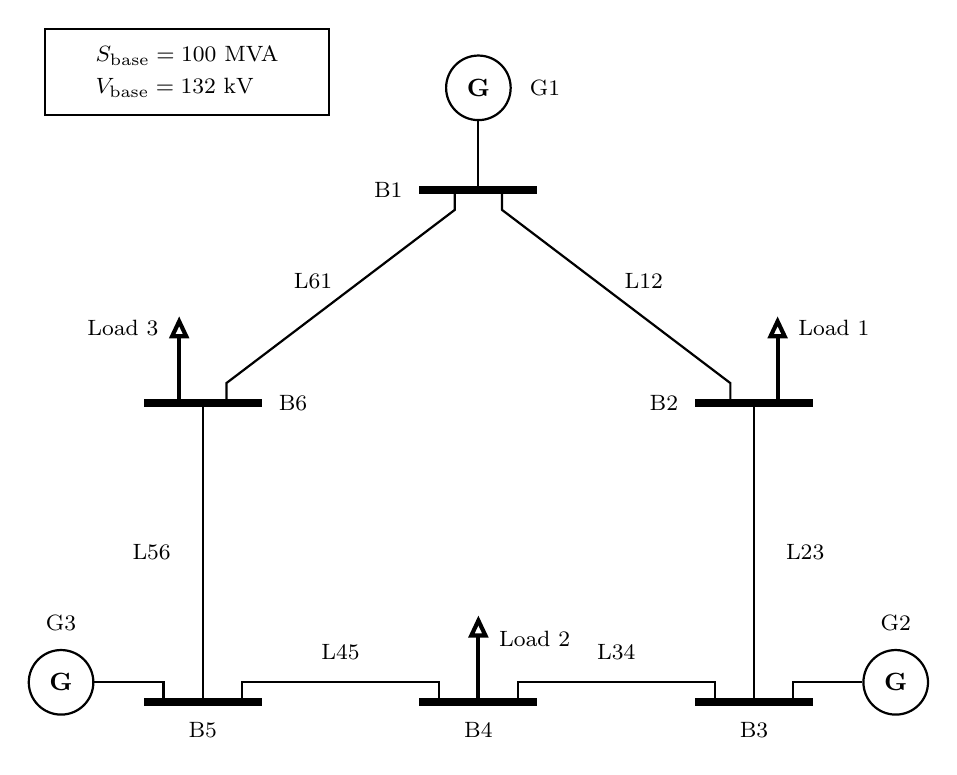
\begin{tikzpicture}[
    bus/.style        = {line width=2.8pt, line cap=rect},
    conductor/.style  = {thick},
    genbox/.style     = {circle, draw, thick, minimum size=0.82cm,
                         inner sep=0pt, font=\small\bfseries},
    % hollow open-triangle load arrow matching original figure
    loadtri/.style    = {-{Triangle[open, length=8pt, width=7pt]},
                         line width=1.5pt},
    lbl/.style        = {font=\small\bfseries, align=center},
    ann/.style        = {font=\footnotesize, align=center},
    linelbl/.style    = {font=\footnotesize, align=center,
                         fill=white, inner sep=1pt},
]

% ============================================================
%  BUS COORDINATES
%   B1 : (5.0,  6.5)   top-centre   (Slack)
%   B2 : (8.5,  3.8)   mid-right    (PQ – Load 1)
%   B3 : (8.5,  0.0)   bottom-right (PV – G2)
%   B4 : (5.0,  0.0)   bottom-centre(PQ – Load 2)
%   B5 : (1.5,  0.0)   bottom-left  (PV – G3)
%   B6 : (1.5,  3.8)   mid-left     (PQ – Load 3)
% ============================================================

% ----------------------------------------------------------
%  BUS 1  –  Slack, G1 above (top-centre)
% ----------------------------------------------------------
% horizontal bus bar
\draw[bus] (4.3, 6.5) -- (5.7, 6.5);
% generator above
\node[genbox] (G1) at (5.0, 7.8) {G};
\draw[conductor] (5.0, 7.4) -- (5.0, 6.5);
\node[ann, right=3pt] at (G1.east) {G1};
% label
\node[ann, left=4pt] at (4.3, 6.5) {B1};

% ----------------------------------------------------------
%  BUS 2  –  PQ, Load 1 (mid-right)
% ----------------------------------------------------------
% vertical bus bar
\draw[bus] (7.8, 3.8) -- (9.2, 3.8);
% hollow-triangle load arrow upward
\draw[loadtri] (8.8, 3.8) -- (8.8, 4.9);
\node[ann, right=4pt] at (8.8, 4.75) {Load 1};
% label
\node[ann, left=4pt] at (7.8, 3.8) {B2};

% ----------------------------------------------------------
%  BUS 3  –  PV, G2 right (bottom-right)
% ----------------------------------------------------------
% horizontal bus bar
\draw[bus] (7.8, 0.0) -- (9.2, 0.0);
% generator to right
\node[genbox] (G2) at (10.3, 0.25) {G};
\draw[conductor] (9.0, 0) -- (9.0, 0.25) -- (G2.west);
\node[ann, above=3pt] at (G2.north) {G2};
% label
\node[ann, below=4pt] at (8.5, 0.0) {B3};

% ----------------------------------------------------------
%  BUS 4  –  PQ, Load 2 (bottom-centre)
% ----------------------------------------------------------
% horizontal bus bar
\draw[bus] (4.3, 0.0) -- (5.7, 0.0);
% hollow-triangle load arrow upward
\draw[loadtri] (5.0, 0.0) -- (5.0, 1.1);
\node[ann, right=4pt] at (5.0, 0.8) {Load 2};
% label
\node[ann, below=4pt] at (5.0, 0.0) {B4};

% ----------------------------------------------------------
%  BUS 5  –  PV, G3 left (bottom-left)
% ----------------------------------------------------------
% horizontal bus bar
\draw[bus] (0.8, 0.0) -- (2.2, 0.0);
% generator to left
\node[genbox] (G3) at (-0.3, 0.25) {G};
\draw[conductor] (G3.east) -- (1.0, 0.25) -- (1.0, 0);
\node[ann, above=3pt] at (G3.north) {G3};
% label
\node[ann, below=4pt] at (1.5, 0.0) {B5};

% ----------------------------------------------------------
%  BUS 6  –  PQ, Load 3 (mid-left)
% ----------------------------------------------------------
% vertical bus bar
\draw[bus] (0.8, 3.8) -- (2.2, 3.8);
% hollow-triangle load arrow upward
\draw[loadtri] (1.2, 3.8) -- (1.2, 4.9);
\node[ann, left=4pt] at (1.2, 4.75) {Load 3};
% label
\node[ann, right=4pt] at (2.2, 3.8) {B6};

% ============================================================
%  TRANSMISSION LINES
% ============================================================

% ---- L61  B6 (1.5, 3.8) ↔ B1 (5.0, 6.5) -----------------
\draw[conductor] (1.8, 3.8) -- (1.8, 4.05) -- (4.7, 6.25) -- (4.7, 6.5);
\node[linelbl] at (2.9, 5.35) {L61};

% ---- L12  B1 (5.0, 6.5) ↔ B2 (8.5, 3.8) -----------------
\draw[conductor] (5.3, 6.5) -- (5.3, 6.25) -- (8.2, 4.05) -- (8.2, 3.8);
\node[linelbl] at (7.1, 5.35) {L12};

% ---- L23  B2 (8.5, 3.8) ↔ B3 (8.5, 0.0) -----------------
\draw[conductor] (8.5, 3.8) -- (8.5, 0.0);
\node[linelbl] at (9.15, 1.9) {L23};

% ---- L34  B3 (8.5, 0.0) ↔ B4 (5.0, 0.0) -----------------
\draw[conductor] (8.0, 0) -- (8.0, 0.25) -- (5.5, 0.25) -- (5.5, 0);
\node[linelbl] at (6.75, 0.63) {L34};

% ---- L45  B4 (5.0, 0.0) ↔ B5 (1.5, 0.0) -----------------
\draw[conductor] (4.5, 0) -- (4.5, 0.25) -- (2.0, 0.25) -- (2.0, 0);
\node[linelbl] at (3.25, 0.63) {L45};

% ---- L56  B5 (1.5, 0.0) ↔ B6 (1.5, 3.8) -----------------
\draw[conductor] (1.5, 0.0) -- (1.5, 3.8);
\node[linelbl] at (0.85, 1.9) {L56};

% ============================================================
%  TITLE – system base (top-left box, matching original style)
% ============================================================
\draw[thick] (-0.5, 8.55) rectangle (3.1, 7.45);
\node[font=\footnotesize, align=left] at (1.3, 8.0)
    {$S_{\text{base}} = 100$ MVA\\[2pt]$V_{\text{base}} = 132$ kV};

\end{tikzpicture}
\end{document}
